%++++++++++++++++++++++++++++++++++++++++
% Don't modify this section unless you know what you're doing!
\documentclass[letterpaper,12pt]{article}
\usepackage{tabularx} % extra features for tabular environment
\usepackage{amsmath}  % improve math presentation
\usepackage[portuguese]{babel}
\usepackage{graphicx} % takes care of graphic including machinery
\usepackage{fancyhdr} % Fancy headers
\usepackage{titling}
\usepackage[margin=1in,letterpaper]{geometry} % decreases margins
\usepackage{cite} % takes care of citations
\usepackage[final]{hyperref} % adds hyper links inside the generated pdf file
\usepackage{xcolor}
\usepackage{booktabs}
\usepackage{amsmath}
\usepackage{amssymb}
\usepackage{booktabs}
\usepackage[table,xcdraw]{xcolor}



\hypersetup{
	colorlinks=true,       % false: boxed links; true: colored links
	linkcolor=black,        % color of internal links
	citecolor=blue,        % color of links to bibliography
	filecolor=magenta,     % color of file links
	urlcolor=blue         
}
%~~~~~~~~~ Page setup
\pagestyle{fancy}
\fancyhf{}
\lhead{PBL Monetária}
\lfoot{Silva, Moraes e Silva}
\rhead{2023}
\rfoot{Page \thepage}
\renewcommand{\footrulewidth}{0.4pt}
%++++++++++++++++++++++++++++++++++++++++
\pagenumbering{gobble} % keep title page without a number

\title{PBL 3 - Monetária }
\author{ \name{João Pedro Miranda da Silva (Noite)\thanks{joao.mirandasilva@ufpe.br}}\\
\name{Paulo Francisco da Silva Júnior  (Manhã)\thanks{paulo.fsilva3@ufpe.br}}\\
\name{Pedro Henrique Aleluia de Moraes (Noite)\thanks{pedro.hamoraes@ufpe.br}}}

\begin{document} 
\date{31 de março de 2023}
\maketitle

\begin{abstract}
Esse documento contém a resolução para o PBL 3 da cadeira de Monetária.
\end{abstract}

\newpage
\pagenumbering{arabic} % start page numbers again
\setcounter{page}{1}

\section{Introdução}
Em primeiro lugar, é importante entender que o risco do investimento, para o investidor, é tão importante quanto o próprio retorno esperado desse ativo. Nesse sentido, buscamos otimizar esses dois fatores, diversificando a carteira de forma que o risco seja mitigado e o retorno dos ativos financeiros se mantenha significantemente alto.
Para que a nossa carteira tenha um parâmetro mais objetivo no que se refere ao risco e  ao retorno esperado, utilizamos de índices e medidas que possibilitam avaliar os investimentos estudados.

\begin{itemize}
    \item \textbf{Retorno Esperado:} Se refere ao ganho de capital esperado para determinado investimento/ativo.
    
    \item\textbf{Índice Sharpe:} O Índice de Sharpe é um indicador que permite uma análise da relação entre o risco e o prêmio de risco de um determinado investimento. 

    \item\textbf{Desvio-padrão do excesso de retorno da carteira:} uma medida importante para verificar a dimensão da incerteza dos ativos financeiros. É importante salientar que o desvio-padrão da taxa de retorno não diferencia boas notícias de más notícias.

    \item\textbf{Prêmio ao risco da carteira:} representa o quanto o investimento de risco rende a mais do que um investimento considerado sem risco. Essa medida pode ser considerada como uma das mais importantes na hora da tomada de decisão dos investidores.

\end{itemize}

\section{Composição da Carteira de Risco}

\subsection{Ambev (ABEV3)}
Fundada em 1999, a Ambev, através de suas subsidiárias, atua na produção, distribuição e comercialização de bebidas e produtos alimentícios. A Ambev opera como subsidiária da Interbrew International B.V.

\subsection{Embraer (EMBR3)}
 Com mais de 50 anos de operações, a Embraer projeta, desenvolve, fabrica e comercializa aeronaves e sistemas no Brasil e internacionalmente. Além disso, a Embraer tornou-se a terceira maior fabricante de jatos comerciais do mundo e líder absoluta no segmento de até 130 assentos.

\subsection{WEG S.A. (WEGE3)}
Fundada em 1961, a WEG é uma das maiores fabricantes de equipamentos elétricos do mundo, atuando na produção e comercialização de bens de capital no Brasil e no exterior. A empresa produz uma gama de componentes industriais para diversos segmentos. Que vão desde motores elétricos, transformadores e turbinas até soluções de energia renovável e de tração elétrica para veículos pesados.

\subsection{Banco do Brasil S.A (BBSA3)}
Sendo o primeiro banco criado em solo brasileiro, o Banco do Brasil S.A, juntamente com suas subsidiárias, oferece produtos e serviços bancários no Brasil e no exterior. Além do segmento bancário, o BB opera no setor de investimentos, gestão de fundos, seguros e outros.

\subsection{Banco da Amazônia (BAZA3)}
O Banco da Amazônia S.A. fornece produtos e serviços bancários na região Norte do Brasil. Sua presença é considerada essencial para o desenvolvimento econômico dos empreendimentos rurais e urbanos dessa região.

\subsection{PetroRio (PRIO3)}
A Petro Rio, com suas subsidiárias, tem como área de atuação a exploração, desenvolvimento e produção de petróleo e gás natural, sendo hoje a maior petroleira privada do Brasil. É uma empresa de capital aberto, além disso, no ano de 2022, possui mais de R\$ 20.3 bilhões em ativos.


\section{Overview da Carteira}

% Please add the following required packages to your document preamble:
% \usepackage{booktabs}

\begin{table}[h!]
\centering
\resizebox{\textwidth}{!}{%
\begin{tabular}{@{}cccccc@{}}
\toprule
\multicolumn{6}{c}{\textbf{Carteira Completa de Ativos}}                 \\ \midrule
\textbf{Ativo} &
  \multicolumn{1}{l}{\textbf{Retorno Anual}} &
  \multicolumn{1}{l}{\textbf{Prêmio ao Risco}} &
  \multicolumn{1}{l}{\textbf{Desvio Padrão}} &
  \multicolumn{1}{l}{\textbf{Índice de Sharpe}} &
  \multicolumn{1}{l}{\textbf{Peso}} \\ \midrule
SELIC                   & 13,75\% & 0       & 0       & 0        & 10\%  \\
ABEV3                   & 4,2\%   & -9,5\%  & 18,4\%  & -0,5191  & 15\%  \\
EMBR3                   & 36,45\% & 22,7\%  & 34,44\% & 0,6591   & 15\%  \\
WEGE3                   & 25,2\%  & 11,45\% & 24,92\% & 0,4595   & 15\%  \\
BBAS3                   & 15,86\% & 2,11\%  & 29,37\% & 0,0721   & 15\%  \\
BAZA3                   & 44,24\% & 30,5\% & 38\% & 0.8017   & 15\%  \\
PRIO3                   & 27,36\% & 13,61\% & 40,68\% & 0,3347   & 15\%  \\ \midrule
\textbf{Carteira Total} & 24,37\%  & 10,62\% & 27,00\% & 0.393503 & 100\% \\ \bottomrule
\end{tabular}%
}
\label{tab:my-table}
\end{table}
\noindent Na composição da nossa carteira, buscamos maximizar os retornos esperados sem abrir mão de minimizar os possíveis riscos de perdas associados. Afim de minimizar os possíveis riscos, buscamos diversificar a carteira com ativos de empresas sólidas e consolidadas no mercado e de setores variados. Algumas dessas empresas são líderes em seus respectivos setores, assim trazendo robustez ao nosso portfólio. Vale ressaltar que os dados utilizados se referem ao período de um ano, sendo  a partir de março de 2022 até março de 2023.\\  

\noindent Como podemos analisar na tabela acima, a nossa carteira possui um elevado índice de retorno anual na faixa dos $24,37\%$ ao ano. Apesar de uma alta volatilidade indicada pelo desvio padrão da nossa carteira, em um cenário pessimista a perda seria pequena quando comparada a um ganho em cenário otimista, tendo como referência média o retorno anual esperado. Optamos também por colocar pesos iguais entre os ativos de risco, o que totaliza $90\%$ da carteira, sendo os restantes $10\%$ em ativo livre de risco (Título do Tesouro Direto SELIC). \\


\begin{figure}[h!]
    \centering
   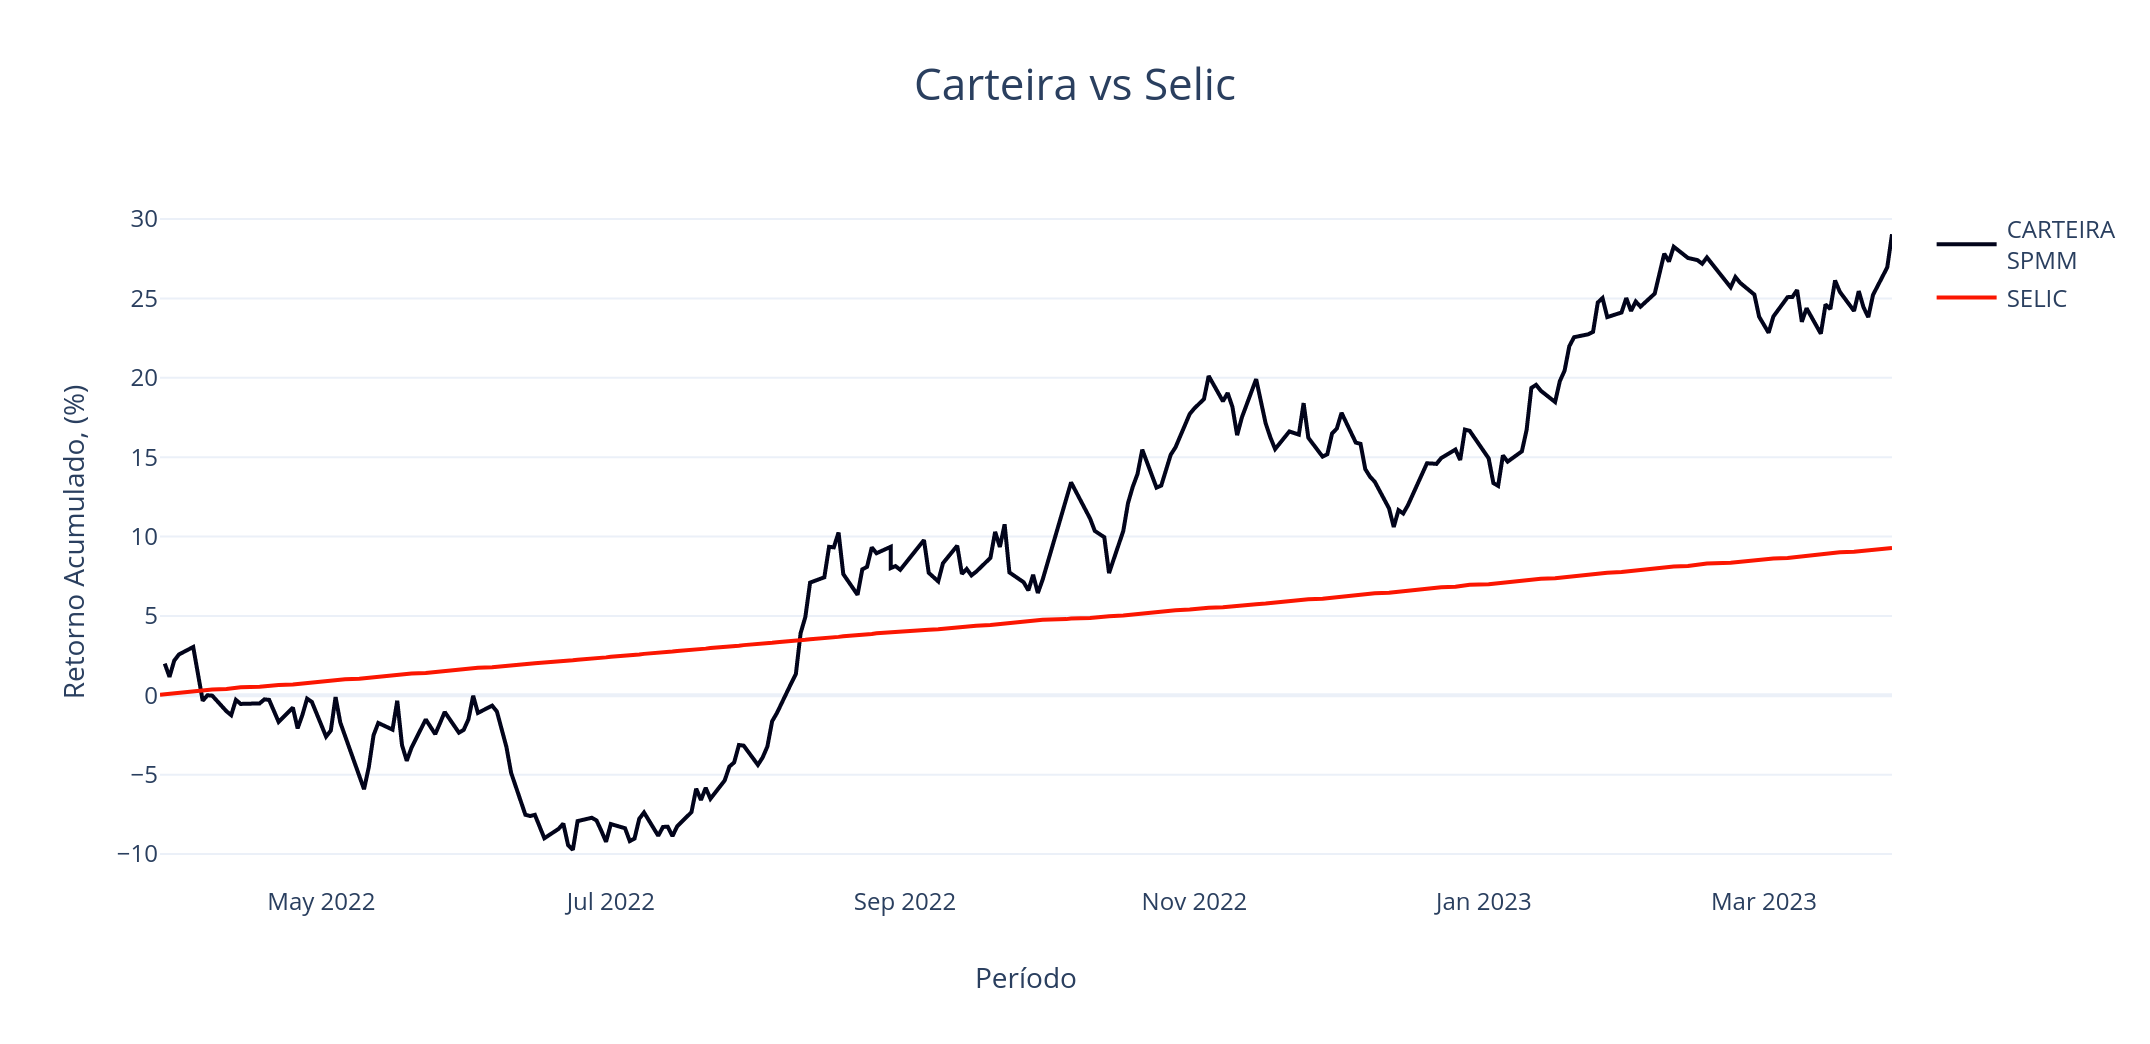
\includegraphics[width=1\columnwidth]{Carteira vs Selic.png}
    \caption{Retorno da carteira comparado ao retorno da SELIC em 12 meses.}
    \label{fig:my_label}
\end{figure}

\noindent Na figura 1, podemos observar o retorno da nossa carteira comparado ao retorno da taxa livre de risco (SELIC). Analisamos que a nossa carteira, nos último 12 meses, possui uma performance superior quando comparada ao ativo livre de risco.

\newpage

\noindent \textbf{{\Large Escolha das Carteiras Ofertadas}}\\

\noindent Primeiramente, iremos listar as carteiras que nos foram oferecidas e que foram consideradas em nosso processo de decisão. Utilizaremos os sobrenomes dos integrantes de cada grupo para listar sua respectiva carteira.

\begin{itemize}
    \item Carteira Ferraz, Madureira, Oliveira, Gasparini e Accioly;
    \item Carteira Eustáquio, Cabral, Pitta, Oscar e Cavalcanti;
    \item Carteira Ribeiro, Lacerda, Dellantonio, Wagner e Neves;
    \item Carteira Dias, Braga, Macedo, Baltar e Guedes;
    \item Carteira Barbosa, Assis, Costa e Thiago.
\end{itemize}

\noindent Dentre as listadas, as duas carteiras que mais nos chamaram a atenção foram as carteiras dos grupos Ferraz \emph{et al.} e Eustáquio \emph{et al.} Porém, entre essas duas carteiras, decidimos por \textcolor{blue}{\textbf{comprar}} a carteira de \textbf{Ferraz \emph{et al.}} e \textcolor{red}{\textbf{rejeitar}} a de \textbf{Eustáquio \emph{et al.}} Para chegar a essa conclusão analisamos as carteiras por seus critérios técnicos e por sua performance passada. Analisamos também a diversificação de cada carteira a fim de mitigar possíveis riscos idiossincráticos dos ativos.\\

\noindent A carteira que decidimos \textcolor{blue}{\textbf{comprar}} é composta por 6 ativos, sendo cinco ativos de risco e um ativo livre de risco. Dentre os ativos de risco, podemos observar a escolha por ativos de empresas líderes de mercado e de alta performance em 12 meses. A carteita possui uma boa diversificação entre setores variados como transporte (Embraer S.A.), financeiro (BB Seguridade), componentes industrias (WEG S.A.), gás e petróleo (Petrobras) e construção (Cury Construtora e Incorporadora). A respeito da análise técnica, observamos elevadas taxas de retorno dentre as quais podemos destacar a da CURY3, com $85,5\%$ de retorno em 12 meses, e do BBSE3, com $48\%$ em 12 meses. Apesar de não terem colocado o retorno carteira em 12 meses, estimamos que seja na casa dos $36\%$. Fizeram também uma projeção dos rendimentos da carteira, o que nos auxiliou no processo de decisão. No geral gostamos da carteira e nos sentimos confortável em alocar os nossos recursos nela.\\

\noindent A carteira que decidimos \textcolor{red}{\textbf{rejeitar}} é composta por cinco ativos, sendo 4 de risco e um livre de risco. Uma diferença importante nessa carteira das demais foi a opção por ativo cambial (dolár), que em cenários de crise, possui boa estabilidade. Porém com instabilidades geopolíticas vindas da guerra da Ucrânia e do atrito com o governo chinês, vemos a exposição direta ao dólar traz consigo um elevado risco no curto e médio prazo. Portanto, optaríamos por outras formas de proteção como comprar ouro e prata no curto prazo. Outro ativo que não nos sentimos confortáveis em ter exposição é VALE3. Apesar de ter boa performance e resultados robustos, avaliamos que os riscos idiossincráticos desse ativo são bastante elevados. Principalmente em relação a baixa manutenção de suas barragens, correndo um risco de gerar um "Brumadinho 2''. Ademais, o fato de não terem colocado o retorno em 12 meses de seus ativos ou até mesmo o o retorno da carteira, dificultou o nosso processo de avaliação da performance da carteira. Eles indicam os preços recomendados de compra e venda segundo análises por especialistas terceiros, os quais não foram sequer citados, o que gera uma desconfiança de nossa parte em suas afirmações.







\end{document}
